\documentclass[12pt,a4paper]{article}
\setlength{\headheight}{14.49998pt}
\addtolength{\topmargin}{-2.49998pt}
\usepackage[utf8]{inputenc}
\usepackage[vietnamese]{babel}
\usepackage{graphicx}
\usepackage{hyperref}
\usepackage{amsmath}
\usepackage{amssymb}
\usepackage[T1]{fontenc}
\usepackage{lmodern}
\usepackage{titlesec}
\usepackage{geometry}
\usepackage{enumitem}
\usepackage{fancyhdr}
\usepackage{xcolor}
\usepackage{listings}
\usepackage{float}
\usepackage{wrapfig}
\usepackage{tikz}
\usepackage{array}
\usepackage{booktabs}
\usepackage{verbatim}
\usepackage{tcolorbox}

% Set margins
\geometry{left=2.5cm, right=2.5cm, top=2.5cm, bottom=2.5cm}

% Define colors
\definecolor{guardianblue}{RGB}{0, 102, 204}
\definecolor{guardiangreen}{RGB}{0, 153, 51}
\definecolor{codecolor}{RGB}{0, 0, 0}
\definecolor{codebackcolor}{RGB}{245, 245, 245}

% Set up code listing style
\lstset{
    backgroundcolor=\color{codebackcolor},
    basicstyle=\footnotesize\ttfamily,
    breaklines=true,
    captionpos=b,
    commentstyle=\color{guardiangreen},
    framexleftmargin=5mm,
    frame=single,
    numbers=left,
    numberstyle=\tiny\color{codecolor},
    keywordstyle=\color{guardianblue},
    showspaces=false,
    showstringspaces=false,
    showtabs=false,
    tabsize=2
}

% Style for titles
\titleformat{\section}
  {\normalfont\Large\bfseries\color{guardianblue}}{\thesection}{1em}{}
\titleformat{\subsection}
  {\normalfont\large\bfseries\color{guardianblue}}{\thesubsection}{1em}{}

% Header and footer
\pagestyle{fancy}
\fancyhf{}
\lhead{GDGOC Hackathon Vietnam 2025}
\rhead{Đội AIGenerated}
\cfoot{\thepage}

\usepackage{hyperref}
\hypersetup{
    colorlinks=true,
    linkcolor=black,    % Changed from guardianblue to black
    filecolor=black,    % Changed from guardianblue to black
    urlcolor=black,     % Changed from guardianblue to black
    citecolor=black,    % Changed from guardianblue to black
    pdfborder={0 0 0},
}

% Cấu hình font chữ cho tiếng Việt
\renewcommand{\rmdefault}{lmr} % Latin Modern Roman
\renewcommand{\sfdefault}{lmss} % Latin Modern Sans
\renewcommand{\ttdefault}{lmtt} % Latin Modern Typewriter

\begin{document}

\begin{titlepage}
\centering

\includegraphics[width=0.5\textwidth]{./Images/guardiannet-logo.png}\\[1cm]
{\Huge\bfseries GuardianNet\\[0.5cm]}
{\large\bfseries Công cụ bảo vệ trực tuyến bằng AI\\[2cm]}

{\large\textbf{Đội AIGenerated}\\[0.5cm]}
{\large\textbf{GDGOC Hackathon Vietnam 2025}\\[2cm]}

\begin{tabular}{rl}
\textbf{Thành viên:} & Nguyễn Hoàn Thiện (Đội trưởng) \\
& Lê Kim Hoàng Trung \\
& Nguyễn Lê Tất Phú \\
& Doãn Cát Phú
\end{tabular}\\[2cm]

\vfill
{\large 12 tháng 4 năm 2025}
\end{titlepage}

\tableofcontents
\newpage

\section{Giới thiệu dự án}

GuardianNet là giải pháp toàn diện nhằm bảo vệ người dùng Internet khỏi những nội dung không phù hợp như hình ảnh bạo lực, khiêu dâm và ngôn từ thô tục. Sản phẩm được phát triển với tiêu chí Responsible AI, nhắm đến việc tạo ra môi trường trực tuyến an toàn, đặc biệt cho trẻ em giúp tạo ra một môi trường Internet an toàn và lành mạnh hơn. Áp dụng công nghệ AI tiên tiến, đặc biệt là phương pháp multi-task learning, cho phép xây dựng mô hình nhận diện chính xác và hiệu quả, đồng thời tích hợp liền mạch vào trình duyệt thông qua extension.

Dựa trên những tiêu chí của một sản phẩm mang tính ``Responsible AI'', GuardianNet đảm bảo:

\begin{itemize}
  \item \textbf{An toàn cho người dùng Internet:} Mục tiêu chính là bảo vệ người dùng, đặc biệt là trẻ em, khỏi tác động tiêu cực của nội dung độc hại, góp phần vào một không gian mạng lành mạnh hơn.

  \item \textbf{Tính công bằng:} Bất kỳ lứa tuổi nào khi truy cập vào Internet, những nội dung độc hại, phản cảm sẽ bị loại bỏ.

  \item \textbf{Tính minh bạch:} Cung cấp cho người dùng (ví dụ: các bậc phụ huynh) khả năng xem lại các nội dung đã bị chặn (nếu cần và đảm bảo riêng tư) và hiểu lý do tại sao chúng bị chặn. Người dùng có thể dễ dàng dùng như một extension trên trình duyệt của mình.

  \item \textbf{Bảo vệ quyền riêng tư và dữ liệu cá nhân của người dùng:} Thông tin được lấy trực tiếp từ trang web để ngăn chặn thông tin độc hại và phản cảm.
\end{itemize}

\section{Vấn đề và phân tích}

\subsection{Xác định vấn đề}

\textbf{Mô tả vấn đề:}

Có thể thấy rằng hiện nay trẻ em và người dùng dễ bị tiếp xúc với nội dung bạo lực và không phù hợp trên Internet, rất nhiều hình ảnh nhạy cảm, 18+, máu me vẫn có thể được truy cập và xem mà không có một biện pháp ngăn chặn nào. Các hệ thống lọc hiện có dựa trên từ khóa hay các tiêu chí cứng nhắc không thể phân biệt đầy đủ các trường hợp phức tạp, dẫn đến cả lỗi bỏ sót lẫn cảnh báo sai. Những hình ảnh đó khi bị cấm cũng dễ dàng xem được bằng nhiều cách khác, những hình ảnh máu me, bạo lực vẫn còn bỏ sót. Tạo nên một môi trường mạng không trong sạch, đặc biệt là với trẻ nhỏ.

\subsection{Phân tích vấn đề}

Có thể thấy thế giới Internet rất rộng lớn, việc dễ dàng tiếp cận với những nội dung không mấy lành mạnh ngay từ khi còn nhỏ có thể dẫn đến những hậu quả nghiêm trọng về tâm sinh lý, nhận thức ảnh hưởng xấu đến quá trình học tập và phát triển. Với người đang gặp các vấn đề tiêu cực hoặc nhân cách bất ổn có thể mắc các vấn đề như trầm cảm, tăng hành vi bạo lực.

Như đã đề cập trước đó, những giải pháp hiện tại còn thiếu tính linh hoạt, vẫn chưa được tập trung giải quyết một cách kỹ lưỡng, không thể cung cấp bảo vệ toàn diện cho các đối tượng nhạy cảm, đặc biệt là trẻ em. Do vậy vẫn còn đó những mối nguy về việc tiếp cận những nội dung bạo lực và nhạy cảm đó.

\section{Giải pháp -- Phương án ứng dụng Responsible AI}

Dựa trên những tiêu chí của Responsible AI và vấn đề về việc quản lý nội dung trên Internet đối với trẻ nhỏ, GuardianNet với vai trò là tiện ích mở rộng trên trình duyệt, tích hợp mô hình AI tiên tiến với phương pháp multi-task learning nhằm tự động quét và xử lý hình ảnh chứa nội dung bạo lực. Bao gồm các đặc trưng như:

\subsection{Quét và phân tích nội dung}

Khi người dùng duyệt web, content script quét các hình ảnh trên trang và gửi dữ liệu về background script. Tại đây, mô hình multi-task learning được sử dụng để xác định:

\begin{itemize}
  \item Hình ảnh có chứa nội dung bạo lực, máu me, nhạy cảm hay không. Nếu có, hình ảnh sẽ bị làm mờ đi hoặc chặn hiển thị.
  
  \item Sự xuất hiện của con người, giúp giảm cảnh báo sai từ các hình ảnh không liên quan (ví dụ: phong cảnh).
\end{itemize}

Ngoài ra, GuardianNet còn quét nội dung văn bản để phát hiện các từ ngữ thô tục, phản cảm, lăng mạ dựa trên danh sách từ khóa và ngữ cảnh câu. Các từ/cụm từ này có thể được ẩn đi hoặc thay thế bằng ký tự [***].

\subsection{Xử lý nội dung tự động}

Khi extension được kích hoạt, những hình ảnh trên web sẽ tự động được load và đưa vào pre-trained model MobileNetV2 kết hợp với mô hình đa tác vụ giúp nhận diện ảnh bạo lực và sự hiện diện của người. Các kết quả của hai nhiệm vụ được mã hóa thành chuỗi nhị phân ``ab''. Với quy tắc:

\begin{itemize}
  \item ``a'' biểu thị kết quả của nhiệm vụ bạo lực (0: không bạo lực, 1: bạo lực).
  
  \item ``b'' biểu thị kết quả của nhiệm vụ phát hiện con người (0: không có người, 1: có người). 
\end{itemize}

Hình ảnh sẽ được quyết định có làm mờ hay không dựa vào mã nhị phân ``ab'', đảm bảo những ảnh an toàn được hiển thị:

\begin{itemize}
  \item ``11'': Bạo lực + có người → Làm mờ.
  
  \item ``10'': Bạo lực + không người → Làm mờ.
  
  \item ``01'': Không bạo lực + không người → Không làm mờ.
\end{itemize}

\subsection{Đảm bảo quyền riêng tư và dữ liệu cá nhân của người dùng}

Hầu hết thông tin sẽ được lấy trực tiếp từ web (bao gồm hình ảnh, văn bản) khi người dùng sử dụng môi trường mạng để có thể ngăn chặn những thông tin tiêu cực và nhạy cảm đó.

\subsection{Báo cáo minh bạch}

Hệ thống ghi lại các hoạt động xử lý nội dung, cung cấp báo cáo định kỳ cho phụ huynh và quản trị viên. Ngoài ra các bậc phụ huynh có thể xem và hiểu lý do tại sao những nội dung đó lại bị chặn, hạn chế con em mình tiếp cận với những nội dung đó một lần nữa.

\section{Chi tiết sản phẩm}

\subsection{Tính năng cốt lõi}

\subsubsection{Nhận diện nội dung bạo lực dưới dạng hình ảnh hoặc văn bản}

Sử dụng mô hình multi-task learning với MobileNetv2 làm base model, hệ thống phân tích hình ảnh theo thời gian thực với hai nhiệm vụ:
\begin{itemize}
  \item Phát hiện nội dung bạo lực.
  \item Phát hiện sự xuất hiện của con người.
\end{itemize}

Kết quả từ hai nhiệm vụ được kết hợp (theo quy tắc nhị phân ``ab'') để xác định chính xác hình ảnh cần làm mờ.

\subsubsection{Cấu hình cá nhân hóa}

Cho phép người dùng tùy chỉnh mức độ nhạy cảm, thiết lập danh sách trắng/đen và cấu hình các tham số báo cáo, đáp ứng nhu cầu riêng của gia đình hoặc môi trường giáo dục.

\subsubsection{Báo cáo và giám sát}

Ghi lại và trình bày báo cáo chi tiết về các hình ảnh đã được xử lý, cung cấp thông tin về thời gian xử lý, số lượng hình ảnh và các thống kê liên quan. Dựa vào đó, phụ huynh có thể xem lý do vì sao những hình ảnh hay text bị chặn để có thể đưa ra biện pháp xử lý.

\subsubsection{Tích hợp liền mạch}

Extension được tích hợp vào các trình duyệt phổ biến (Chrome, Edge, Brave) với giao diện người dùng trực quan và dễ sử dụng, đảm bảo quá trình duyệt web không bị gián đoạn.

\subsection{Giao diện người dùng \& Tài liệu hướng dẫn sử dụng}

\subsubsection{Giao diện}

Giao diện người dùng của GuardianNet được thiết kế đơn giản, trực quan với các thành phần:
\begin{itemize}
  \item Pop-up hiển thị trạng thái của bộ lọc.
  \item Trang Options cho phép điều chỉnh cấu hình và xem báo cáo.
\end{itemize}

\subsubsection{Hướng dẫn sử dụng}

\textbf{Các bước cài đặt extension:}

\paragraph{Bước 1: Chuẩn bị extension}\mbox{}

\begin{lstlisting}[language=bash,
                   inputencoding=utf8,
                  extendedchars=true,
                  literate={đ}{{d}}1]
 # 1. Clone repository
 git clone https://github.com/Thiennguyen21it/GDGOC-hackathon-2025-AIGenerated.git
 
 # 2. Install dependencies
 npm install
 
 # 3. Build extension
 npm run build

 # 4. Go to the directory to load the extension:
 cd build/chrome-mv3-dev
\end{lstlisting}
                

Hoặc tải File zip mà chúng tôi cung cấp tại: \\ 
\url{https://drive.google.com/drive/folders/16-LkgX4iaxwfhx7ZY1gF1DSYc4VG1HSr}, giải nén để tiếp tục các bước sau.

\paragraph{Bước 2: Load extension vào Chrome:}\mbox{}

1. Truy cập chrome://extensions/

\begin{figure}[H]
  \centering
  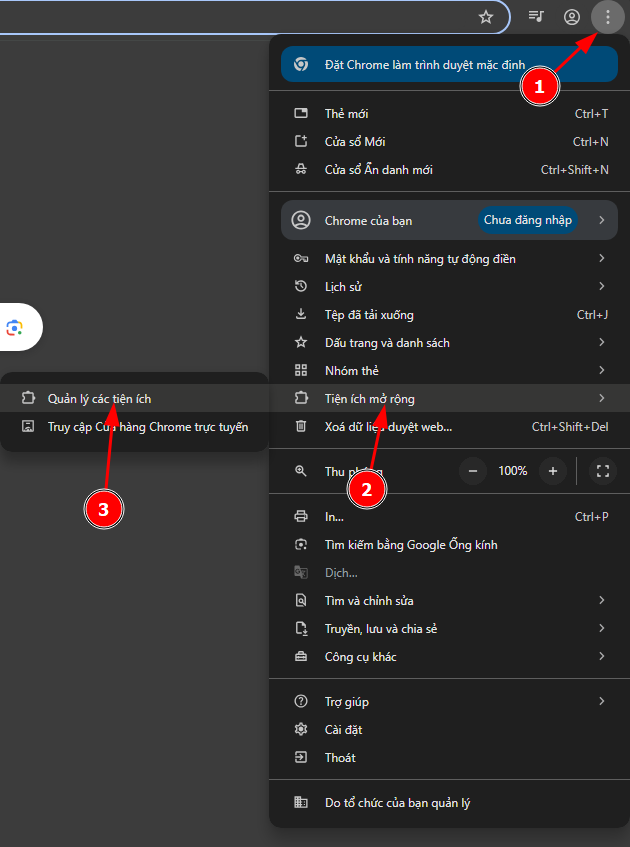
\includegraphics[width=0.7\textwidth]{./Images/image1.png}
  \caption{Trang Extensions của Chrome}
\end{figure}

2. Bật ``Chế độ nhà phát triển''

\begin{figure}[H]
  \centering
  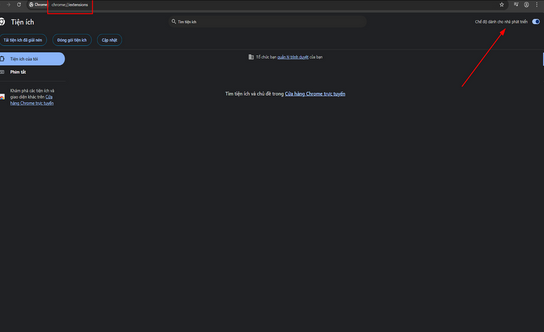
\includegraphics[width=0.8\textwidth]{./Images/image2.png}
  \caption{Kích hoạt chế độ nhà phát triển}
\end{figure}

3. Click ``Tải tiện ích đã giải nén''

\begin{figure}[H]
  \centering
  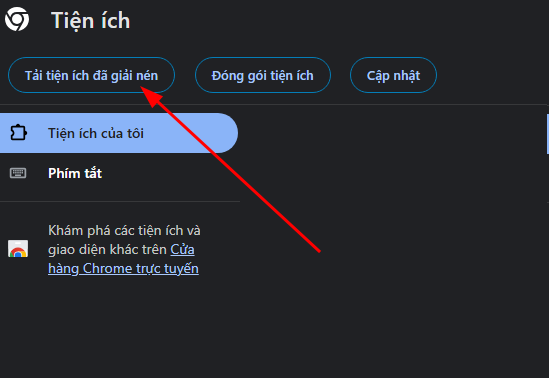
\includegraphics[width=0.8\textwidth]{./Images/image3.png}
  \caption{Tải extension đã giải nén}
\end{figure}

4. Chọn thư mục build của project

\begin{figure}[H]
  \centering
  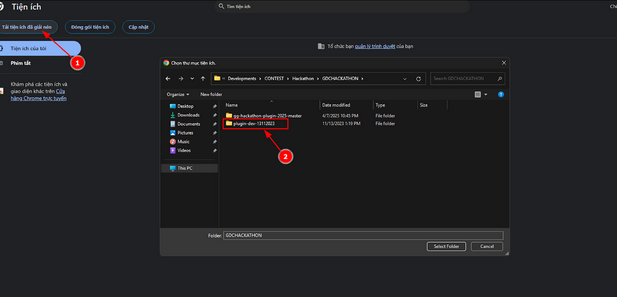
\includegraphics[width=0.9\textwidth]{./Images/image6.png}
  \caption{Chọn thư mục build}
\end{figure}

5. Extension đã load thành công!

\begin{figure}[H]
  \centering
  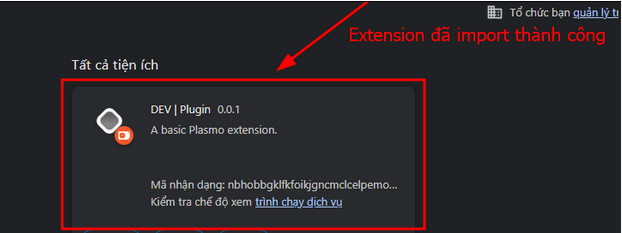
\includegraphics[width=0.9\textwidth]{./Images/image4.png}
  \caption{Extension đã cài đặt thành công}
\end{figure}

Giờ bạn có thể bật extension và test thử bằng cách truy cập những trang chứa nội dung nhạy cảm, bạo lực,...

\begin{figure}[H]
  \centering
  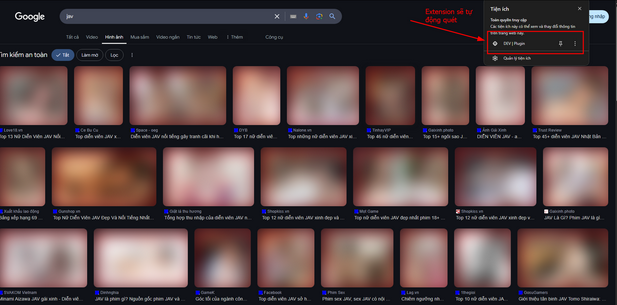
\includegraphics[width=0.9\textwidth]{./Images/image7.png}
  \caption{Giao diện extension khi kích hoạt}
\end{figure}

\section{Biểu đồ kiến trúc và công nghệ}

\begin{figure}[H]
  \centering
  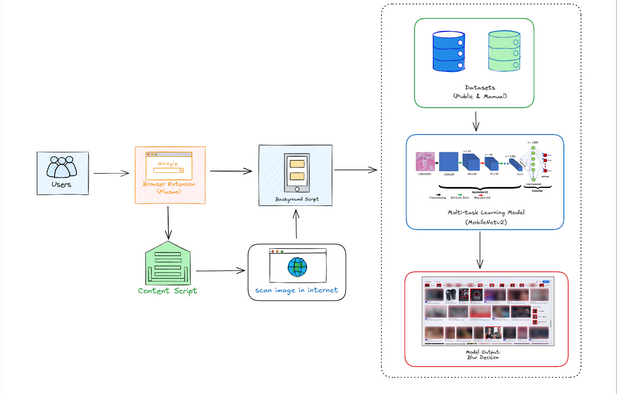
\includegraphics[width=0.9\textwidth]{./Images/image8.png}
  \caption{Kiến trúc tổng thể của GuardianNet}
\end{figure}

\subsection{Kiến trúc hệ thống \& Mô hình AI}

\subsubsection{Multi-task Learning Model}

Học đa tác vụ giúp huấn luyện model học được nhiều tác vụ liên quan với nhau cùng lúc, không như model đơn tác vụ chỉ có thể học một tác vụ duy nhất. Bằng cách cho model học đa tác vụ, nó có thể học những đặc trưng chung có từ nhiều tác vụ liên quan, giúp tăng cường nhận diện hình ảnh bạo lực. Với 2 tác vụ:

\begin{itemize}
  \item Phát hiện nội dung bạo lực.
  \item Phát hiện sự xuất hiện của con người.
\end{itemize}

\subsubsection{Base Model} 

Mô hình học đa tác vụ gồm base model là MobileNetv2 sử dụng các phép tích chập có thể tách theo chiều sâu để xây dựng các mô hình nhẹ với chi phí tính toán giảm so với các phép tích chập tiêu chuẩn. MobileNetv2 đã được huấn luyện trước trên ImageNet, đảm bảo kích thước nhỏ và hiệu năng cao.

\subsubsection{Các tác vụ được huấn luyện}

Gồm có 2 tác vụ:
\begin{itemize}
  \item Phát hiện hình ảnh mang nội dung bạo lực.
  \item Phát hiện sự xuất hiện của con người.
\end{itemize}

\subsubsection{Kết hợp kết quả} 

Sử dụng quy tắc nhị phân ``ab'' để đưa ra quyết định cuối cùng: làm mờ nếu nhận nhãn ``11'' (có bạo lực và có sự xuất hiện của con người).

\subsection{Tích hợp vào Web Extension}

\subsubsection{Framework Plasmo}

Extension được xây dựng trên nền tảng Plasmo, một framework hiện đại giúp phát triển các tiện ích mở rộng cho trình duyệt một cách nhanh chóng, dễ bảo trì và tối ưu hiệu năng.

\subsubsection{Cấu trúc Extension}

\begin{itemize}
  \item \textbf{Manifest V3:} Định nghĩa quyền truy cập, background script và content script.
  
  \item \textbf{Background Script:} Quản lý tải mô hình và xử lý yêu cầu từ content script.
  
  \item \textbf{Content Script:} Quét các hình ảnh trên trang, gửi dữ liệu về background và áp dụng hiệu ứng làm mờ khi cần.
\end{itemize}

\subsection{Công nghệ và công cụ hỗ trợ}

\subsubsection{Ngôn ngữ \& Frameworks}

\begin{itemize}
  \item \textbf{Python:} Dùng để huấn luyện mô hình AI với TensorFlow và Keras.
  
  \item \textbf{MobileNetv2:} Là kiến trúc chính cho mô hình đa tác vụ.
  
  \item \textbf{JavaScript, HTML5, CSS3:} Sử dụng cùng với Plasmo để xây dựng giao diện và tích hợp extension.
\end{itemize}

\subsubsection{API \& Dịch vụ}

\begin{itemize}
  \item \textbf{Chrome Extensions API:} Để tích hợp mô hình và xử lý hình ảnh trực tiếp trên trình duyệt.
\end{itemize}

\subsubsection{Datasets}

Kết hợp dữ liệu từ các bộ dữ liệu công khai (Real Life Violence Situations Dataset, HAR Dataset) và dữ liệu thu thập thủ công từ các nền tảng xã hội, đảm bảo tính đa dạng và thực tế trong huấn luyện mô hình.

\section{Các công cụ, Dependencies, Frameworks và Datasets}

\subsection{Dependencies và Frameworks}

\begin{itemize}
  \item \textbf{Front-End:} JavaScript, HTML5, CSS3. Framework Plasmo để phát triển extension.
  
  \item \textbf{AI/ML:} Python, TensorFlow, Keras, MobileNetv2.
\end{itemize}

\subsection{Datasets}

\begin{itemize}
  \item \textbf{Hình ảnh:} Dữ liệu công khai kết hợp với dữ liệu thu thập thủ công từ các nguồn xã hội.
  
  \item \textbf{Văn bản \& Danh sách từ khóa:} Hỗ trợ việc xử lý ngữ cảnh và tăng độ chính xác nhận diện.
\end{itemize}

\subsection{Công cụ hỗ trợ}

\begin{itemize}
  \item \textbf{API:} Chrome Extensions API
  
  \item \textbf{Quản lý dự án:} Git, GitHub, và các công cụ hỗ trợ phát triển khác.
\end{itemize}

\section{Kế hoạch phát triển \& Tiềm năng mở rộng}

\subsection{Kế hoạch phát triển}

\subsubsection{Giai đoạn 1 (Hackathon)}

\begin{itemize}
  \item Phát triển phiên bản MVP với chức năng quét và xử lý hình ảnh cơ bản thông qua mô hình đa tác vụ.
  
  \item Đảm bảo giao diện và hướng dẫn sử dụng thân thiện, dễ tiếp cận cho người dùng thử nghiệm.
\end{itemize}

\subsubsection{Giai đoạn 2 (Sau Hackathon)}

\begin{itemize}
  \item Nâng cao độ chính xác của mô hình AI, bổ sung các chức năng báo cáo chi tiết và cấu hình nâng cao.
  
  \item Tích hợp thêm các cơ chế bảo mật và quản trị người dùng nhằm tăng cường tính minh bạch.
\end{itemize}

\subsubsection{Giai đoạn 3 (Phát triển dài hạn)}

\begin{itemize}
  \item Mở rộng ứng dụng sang nhiều nền tảng (mobile, desktop) và đối tượng sử dụng (trường học, doanh nghiệp, gia đình).
  
  \item Nghiên cứu tích hợp thêm các công nghệ như deepfake detection, nhận diện ngữ cảnh nâng cao để mở rộng phạm vi bảo vệ.
\end{itemize}

\subsection{Tiềm năng mở rộng}

\textbf{Ứng dụng đa dạng:} GuardianNet có thể được áp dụng trong các môi trường gia đình, trường học và các tổ chức nhằm bảo vệ trẻ em và người dùng khỏi nội dung không phù hợp.

\textbf{Khả năng thị trường:} Với xu hướng ngày càng tăng của việc tiêu thụ nội dung trên Internet và nhu cầu bảo vệ người dùng, sản phẩm có tiềm năng mở rộng ra nhiều quốc gia và lĩnh vực khác nhau.

\section{Kết luận}

GuardianNet là giải pháp toàn diện ứng dụng công nghệ AI tiên tiến kết hợp phương pháp multi-task learning để nhận diện và lọc bỏ nội dung bạo lực trên Internet. Sản phẩm không chỉ đạt độ chính xác cao (98.5\%) mà còn tích hợp liền mạch vào trình duyệt, giúp tạo ra môi trường duyệt web an toàn và thân thiện cho trẻ em. Với tiêu chí Responsible AI, GuardianNet cam kết về sự công bằng, minh bạch, bảo mật và khả năng mở rộng trong tương lai.

\section*{Tài liệu tham khảo}
\begin{itemize}
  \item TensorFlow: \url{https://www.tensorflow.org/}
  \item Keras: \url{https://keras.io/}
  \item MobileNetV2 (TensorFlow Guide): \url{https://www.tensorflow.org/api_docs/python/tf/keras/applications/MobileNetV2}
  \item Plasmo Framework: \url{https://docs.plasmo.com/}
  \item Chrome Extensions API: \url{https://developer.chrome.com/docs/extensions/reference/}
\end{itemize}


\section{Thông tin liên hệ}

\begin{tcolorbox}[colback=white, colframe=guardianblue, arc=3mm, title=Thông tin liên hệ đội AIGenerated]
\begin{tabular}{@{}p{4.5cm}|p{8cm}@{}}
\textbf{Nguyễn Hoàn Thiện (Leader)} & 
Email: thiennh.21it@vku.udn.vn \\
& SĐT: 0356496977 \\
\midrule
\textbf{Lê Kim Hoàng Trung (Member)} & 
Email: trunglkh.21it@vku.udn.vn \\
& SĐT: 0962043095 \\
\midrule
\textbf{Nguyễn Lê Tất Phú (Member)} & 
Email: phunlt.21it@vku.udn.vn \\
& SĐT: 0522944603 \\
\midrule
\textbf{Doãn Cát Phú (Member)} & 
Email: phudc.21it@vku.udn.vn \\
& SĐT: 0935026145 \\

\end{tabular}
\end{tcolorbox}

\end{document}


